\PassOptionsToPackage{usenames,dvipsnames,svgnames,table}{xcolor}
%\RequirePackage{atbegshi}
\documentclass[mathserif, xcolor=svgnames]{beamer}
\usepackage{eulervm}
\usepackage[latin1]{inputenc}
\usetheme{Dresden}
%\usetheme{Berkeley}
%\usetheme{Darmstadt}
\usecolortheme[named=DarkRed]{structure}
\setbeamertemplate{items}[default]
\setbeamertemplate{blocks}[rounded][shadow=true]
\usepackage{booktabs}
\usepackage{dcolumn}
\newcolumntype{.}{D{.}{.}{-1}}
\setbeamercovered{transparent}
\usepackage{graphicx}
\usepackage{amssymb}
\usepackage{epstopdf}
\usepackage{ulem}
\usepackage{fancybox}
\usepackage{setspace}
\usepackage{multicol}
\setbeameroption{show notes}
\logo{
\includegraphics[height=1cm]{bucky.pdf}}



\newtheorem{question}{Questions}
\title{Beamer Basics}
\subtitle{\LaTeX Workshop 2}
\author{Sarah B. Bouchat \\ University of Wisconsin}

\date{\today}
\begin{document}
% Notes
% Needs pictures "bucky" "pid_0009_gallup.pdf"
% Needs packages {fancybox} {multicol} {colortbl}

\begin{frame}[plain]
\titlepage
\vspace{.25in}
\hyperlink{hyper}{\beamergotobutton{Return}}\\
\begin{center}
\tiny{This handout borrows heavily from the department's 2010 \LaTeX~handout and Simon Haeder's previous Beamer working example}
\end{center}
\end{frame}

\section{Beginning Beamer}
\subsection{}
\begin{frame}[fragile, label=second]{Getting Beamer}{Beamer Me Up, Scotty!}
To use Beamer, you must obtain the beamer document class and several packages.  These can be downloaded at:

\vspace{10pt}

\verb+http://sourceforge.net/projects/latex-beamer/+

\vspace{10pt}
WinEdt should be able to automatically download any missing packages. MikTeX also has them.
\vspace{1.5in}

\hyperlink{hyper}{\beamergotobutton{Return}}
\end{frame}

\begin{frame}[fragile, label=third]{How Beamer Works}
Beamer functions much like any other \LaTeX  document, but it has its own special document class
\begin{verbatim}
\documentclass{beamer}
\end{verbatim}

Many of the commands remain the same, but some may vary.  In many cases, however, you are able to simply copy and paste things from your other \LaTeX documents right into Beamer with only minor reformatting.

\end{frame}



\begin{frame}[fragile, label=fourth]{Class (Warfare) Options}
Just like for other document classes, Beamer has several options:

\begin{itemize}
\item Font sizes \verb+[10pt]+
\item Transparencies \verb+[trans]+
\item Handouts \verb+[handout]+
\end{itemize}
\vspace{10pt}
\textbf{Example:}
\begin{verbatim}
\documentclass[handout]{beamer}
\end{verbatim}

\end{frame}


\section{Keeping Up Appearances}
\begin{frame}[fragile, label=fifth]{Themes}
Beamer comes a variety of presentation themes or design templates.

\vspace{10pt}

\verb+\usetheme{Hannover}+

\vspace{10pt}

These will automatically create the style features of your presentation. . . . \pause  You \textit{can} build your own themes.

\end{frame}

\subsection{Themes}
\begin{frame}[fragile]{Themes}
Want to see these in action? Go to \verb+http://www.hartwork.org/beamer-theme-matrix/+

\begin{block}{Available Themes}
\begin{multicols}{3}
\begin{itemize}
\item Antibes
\item Bergen 
\item Berkeley 
\item Berlin
\item Boadilla 
\item Copenhagen 
\item Darmstadt 
\item Dresden
\item Frankfurt 
\item Goettingen 
\item Hannover 
\item Ilmenau
\item Juanlespins 
\item Madrid 
\item Malmoe 
\item Marburg
\item Montpellier 
\item Paloalto 
\item Pittsburgh 
\item Rochester
\item Singapore
\end{itemize}
\end{multicols}
\end{block}
\end{frame}



\begin{frame}[fragile, label=sixth]{Colors}
Beamer allows you to set the color for all elements in your frames.
\vspace{15pt}

You can either create your own color scheme:

\verb+\usecolortheme[rgb={0,.5,.5}]{structure} +

\vspace{10pt}

Or use a pre-packaged one:

\verb+\usecolortheme{seagull}+

\end{frame}
\subsection{Colors}
\begin{frame}{Color Themes}


\begin{block}{Available Color Themes}
\begin{multicols}{2}
\begin{itemize}
\item albatross 
\item crane 
\item beetle 
\item dove
\item fly 
\item seagull 
\item wolverine
\item beaver
\end{itemize}
\end{multicols}
\end{block}
These are also available for viewing on the aforementioned Beamer Theme Matrix.
\end{frame}



\subsection{Fonts}
\begin{frame}[fragile]{Fonts}
Beamer allows you to set the font for your document.
\vspace{10pt}
Beamer's default font is sans serif. But you can change that:
\verb+\usefonttheme{serif}+

You can also set separate fonts for different functions. For example:

\verb+\documentclass[mathserif, xcolor=svgnames]{beamer}+
\verb+\usepackage{eulervm}+

\end{frame}

\begin{frame}[fragile]{Innies Versus Outies}
You can also modify both the inner and the outer themes and colors.

\begin{itemize}
\item<2 -> Inner themes and colors refer to things inside the frames
\item<3 -> Outer themes and colors refer to the headline, footline, sidebars, logo, and frame title
\end{itemize}



\end{frame}

\subsection{Inner and Outer}
\begin{frame} {Inner and Outer Themes}
\begin{columns}[t]
\column{.5\textwidth}
\begin{block}{Inner Color Themes}
\begin{itemize}
\item lily
\item orchid
\item rose
\end{itemize}
\end{block}
\column{.5\textwidth}
\begin{block}{Outer Color Themes}
\begin{itemize}
\item whale
\item seahorse
\item dolphin
\end{itemize}
\end{block}
\end{columns}
\end{frame}


\section{The Frames}

\begin{frame}[fragile]{Framing Your Argument}
Here's what a basic Beamer frame looks like:

\begin{verbatim}

\begin{frame}[option] {Title} {Subtitle}

Stuff goes in here
\end{verbatim}
\verb+\end{frame}+

\end{frame}


\begin{frame}[fragile]{A Frame Divided}
You can divide a frame into two separate columns using the columns environment.

\begin{scriptsize}
\begin{verbatim}

\begin{frame}
\begin{columns}

\begin{column}{5cm}
This stuff will appear in the first column.
\end{column}

\begin{column}{5cm}
This stuff will appear in the second column.
\end{column}

\end{columns}
\end{verbatim}

\verb+\end{frame} +
\end{scriptsize}

\end{frame}


\section{Inside the Frame}
\begin{frame}[label=list]{What kinds of things can go into frames?}
\begin{itemize}
\item<1-> Text
\item<2-> Lists/Bullet points
\item<3-> Tables
\item<4-> Figures
\item<5 -> Equations
\item<6-> Movies
\item<7-> Bucky
\item<8-> Puppies
\end{itemize}
\vspace{1in}

\hyperlink{hyper}{\beamergotobutton{Return}}
\end{frame}

\begin{frame}[label=list]{What kinds of things can go into frames?}
\begin{itemize}
\item\alert<1-> {Text}
\item\alert<2-> {Lists/Bullet points}
\item\alert<3-> {Tables}
\item\alert<4-> {Figures}
\item\alert<5 ->{Equations}
\item\alert<6->{Movies}
\item\alert<7-> {Bucky}
\item\alert<8-> {Puppies}
\end{itemize}
\vspace{1in}

\hyperlink{hyper}{\beamergotobutton{Return}}
\end{frame}


\begin{frame}{What kinds of things can go into frames?}

\begin{itemize}
\item Text
\item Lists/Bullet points
\item Tables
\item Figures
\item Equations
\item Movies
\item Bucky
\item \sout{Puppies}
\end{itemize}
\end{frame}

\begin{frame}[fragile]{Beamer's List}
Lists or bullet points in Beamer work just the same as in other documents.

\begin{itemize}
\item Itemize environment
\item Enumerate environment
\item Describe environment
\end{itemize}

But you can also number your items so they appear one at a time
\begin{itemize}
\item<2> This one will be highlighted \verb+\item<1>+
\item<3> Wait?  Where did the first one go? \verb+\item<1>+
\end{itemize}

Or have them revealed one at a time
\begin{itemize}
\item<4-> Let the suspense build . . . \verb+\item<1 ->+
\item<5 -> then reveal your brilliance \verb+\item<2 ->+
\end{itemize}

The numbering tells Beamer when the bullet will appear.

\end{frame}

\begin{frame}{A Side Note on the Description Environment}
\begin{description}[Second Item]
\item[First Item] Description of first item
\item[Second Item] Description of second item
\item[Third Item] Description of third item
\item[Forth Item] Description of forth item
\end{description}
\end{frame}

\begin{frame}[fragile]{Example City (for all your example needs)}
Matt's To Do List:
\begin{columns}

\begin{column}{2in}
\begin{enumerate}
\item<2 -> Bike for salvation
\item<3 -> Shower my sins away
\item<6 -> Work on dissertation
\begin{enumerate}
\item<7 -> Feel more depressed
\end{enumerate}
\item<4 -> Have awkward meeting with adviser
\begin{enumerate}
\item<5 -> Feel depressed
\end{enumerate}
\item<8 -> Drink sorrows away
\item<8 -> Sleep/Pass out
\item<8 -> Repeat
\end{enumerate}
\end{column}

\begin{column}{2in}
\begin{scriptsize}
\begin{verbatim}
\begin{enumerate}
\item<2 -> Bike for salvation
\item<3 -> Shower my sins away
\item<6 -> Work on dissertation
\begin{enumerate}
\item<7 -> Feel more depressed
\end{enumerate}
\item<4 -> Have awkward meeting with adviser
\begin{enumerate}
\item<5 -> Feel depressed
\end{enumerate}
\item<8 -> Drink sorrows away
\item<8 -> Sleep/Pass out
\item<8 -> Repeat
\end{enumerate}
\end{verbatim}
\end{scriptsize}
\end{column}
\end{columns}

\end{frame}


\begin{frame}[fragile, plain]{Tables}
\begin{columns}

\begin{column}{2in}
\singlespacing
\begin{center}  \begin{small}
\begin{tabular}{rrrr} \addlinespace[5pt] \toprule[1.5pt]
\multicolumn{1}{c}{$x_i$} & \multicolumn{1}{c}{$\bar{x}$} &
\multicolumn{1}{r}{$x_i - \bar{x}$} & $(x_i - \bar{x})^2$\\ \midrule
62 & 54.9 & 7.1 & 50.41 \\
53 &  54.9 & -1.9 & 3.61 \\
81&  54.9 & 26.1 & 681.21 \\
47 &  54.9 & -7.9 & 62.41 \\
56 &  54.9 & 1.1 & 1.21 \\
39 &  54.9 & -15.9 & 252.81 \\
45 &  54.9 & -9.9 & 98.01 \\
59 &  54.9 & 4.1 & 16.81 \\
47 &  54.9 & -7.9 & 62.41 \\
60 &  54.9 & 5.1 &  26.01 \\
\midrule
\multicolumn{1}{c}{$\sum$} & & 0 & 1254.9\\
\bottomrule[1.5pt] \addlinespace[5pt]
 \end{tabular} \end{small} \end{center}
\end{column}

\begin{column}{2in}
\begin{scriptsize}
\begin{verbatim}
\begin{center}  \begin{small}
\begin{tabular}{rrrr} \addlinespace[5pt] \toprule[1.5pt]
\multicolumn{1}{c}{$x_i$} & \multicolumn{1}{c}{$\bar{x}$} &
\multicolumn{1}{r}{$x_i - \bar{x}$} & $(x_i - \bar{x})^2$\\ \midrule
62 & 54.9 & 7.1 & 50.41 \\
53 &  54.9 & -1.9 & 3.61 \\
81&  54.9 & 26.1 & 681.21 \\
47 &  54.9 & -7.9 & 62.41 \\
56 &  54.9 & 1.1 & 1.21 \\
39 &  54.9 & -15.9 & 252.81 \\
45 &  54.9 & -9.9 & 98.01 \\
59 &  54.9 & 4.1 & 16.81 \\
47 &  54.9 & -7.9 & 62.41 \\
60 &  54.9 & 5.1 &  26.01 \\
\midrule
\multicolumn{1}{c}{$\sum$} & & 0 & 1254.9\\
\bottomrule[1.5pt] \addlinespace[5pt]
 \end{tabular} \end{small} \end{center}
 \end{verbatim}
 \end{scriptsize}
\end{column}

\end{columns}
\end{frame}

\begin{frame}{Blocks}
\begin{block}{Introduction to {\LaTeX}}
"Beamer is a {\LaTeX}class for creating presentations that are held using a projector..."
\end{block}
\end{frame}

\begin{frame}{Other Block Environments}
\begin{block}{Other Block Environments}
\begin{tabular}{l|l} 
\textbf{Content Type} & \textbf{Corresponding Environment}\\\hline
\textbf{Generic} & block\\
\textbf{Theorems} & theorem\\
\textbf{Lemmas} & lemma\\
\textbf{Proofs} & proof\\
\textbf{Corollaries} & corollary\\
\textbf{Examples} & example\\
\textbf{Highlighted Title} &alertblock\\
\end{tabular}
\end{block}
\end{frame}

\begin{frame}[fragile]{Defining Your Own Block Environment}
As with basically everything else in \LaTeX and Beamer, you can define your own block environment.
\vspace{10pt}
%\verb+\newtheorem{question}{Questions}+
%\vspace{10pt}
\begin{question}
My research question??
\end{question}
\vspace{10pt}
\verb+\newtheorem{ex}{Example}+
\verb+\newtheorem{hyp}{Hypotheses}+
\end{frame}

\begin{frame}{Using Blocks and Columns}
\begin{columns}[t]
\column{.5\textwidth}
\begin{block}{Column 1 Header}
Column 1 Body Text
\end{block}
\column{.5\textwidth}
\begin{block}{Column 2 Header}
Column 2 Body Text
\end{block}
\end{columns}
\end{frame}

\begin{frame}{Text Boxes}

\shadowbox{Sample Text}\\
\begin{flushright}
\fbox{Sample Text}\\
\end{flushright}
\begin{center}
\doublebox{Sample Text}\\
\end{center}
\begin{flushleft}
\ovalbox{Sample Text}\\
\end{flushleft}
\begin{center}
\Ovalbox{Sample Text}\\
\end{center}

\end{frame}


\begin{frame}[fragile, label=figs]{Figures}

\begin{figure}[h!]
   \centering
       \caption{Party Identification, 2000-2009}
    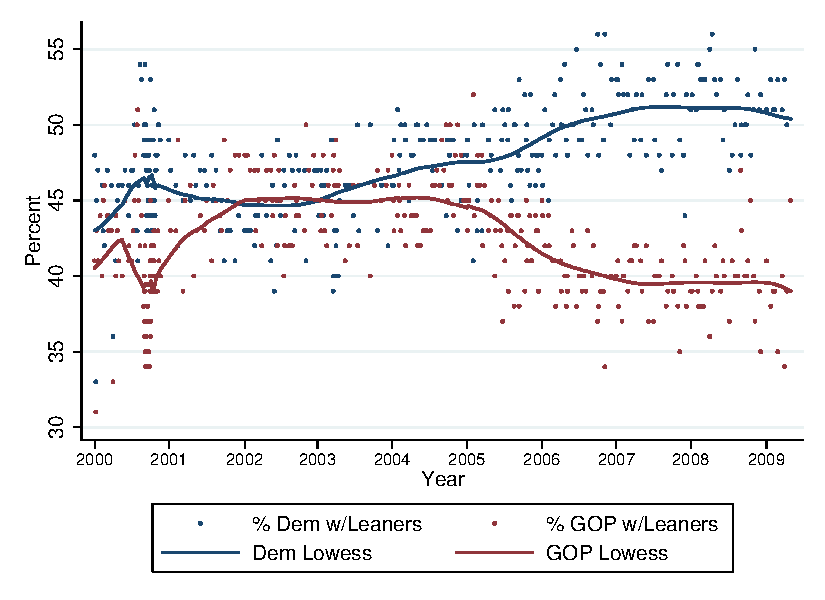
\includegraphics[width=3.5in]{pid_0009_gallup.pdf}
    \end{figure}

\vspace{-22pt}
\hyperlink{hyper}{\beamergotobutton{Return}}
\end{frame}

\begin{frame}[fragile]{Figures}

\begin{verbatim}
\begin{figure}[h!]
   \centering
       \caption{Party Identification, 2000-2009}
    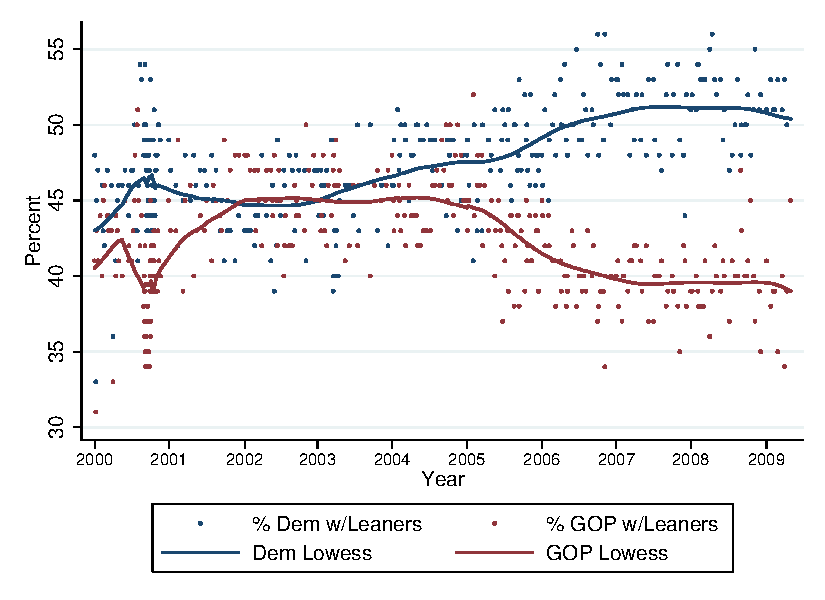
\includegraphics[width=3.5in]{pid_0009_gallup.eps}
    \end{figure}
\end{verbatim}

\end{frame}

\begin{frame}[fragile]{Equations}
You are use the equations environment in Beamer just like in other documents.

\begin{equation}
p(A|B)=\frac{p(A)}{p(B)}p(B|A)
\end{equation}
\vspace {10pt}

You can also do neat stuff using the block environment.

\begin{block}{An Equation in a Box!}
\begin{equation}
p(A|B)=\frac{p(A)}{p(B)}p(B|A)
\end{equation}
\end{block}

\end{frame}

\begin{frame}[fragile]{Logos}
How did I get Bucky to appear in every frame?

\vspace{10pt}

\verb+ \logo{
\includegraphics[height=2cm]{bucky}} +

\end{frame}

\begin{frame}[fragile]{Note to Self}
You can include notes to yourself about particular slides or parts of slides.
\vspace{11pt}

\verb+\note[option]{notetext}+
\vspace{11pt}

Your notes will not appear unless you tell them to appear.  In the preamble, include \verb+ \setbeameroption{show notes} + in your preamble, and the notes will appear on a separate slide immediately following.

\begin{itemize}
\item<2-> Cultural Anthropologists
\item<3-> Political Scientists
\item<4-> Economists
\note[item]<4>{Tell joke about economists.}
\note[item]<4>{Make it short.}
\note[item]<4>{Pause for laughter.}
\end{itemize}

\end{frame}


\begin{frame}[fragile, label=hyper, plain]{Hyperlinks}{What happens when your links have too much sugar}
You can add hyperlinks to your presentations to allow for nonlinear jumps in your presentations.
\vspace{11pt}

\verb+ \begin{frame}[label=targetname] +

\verb+ \hyperlink{targetname}{text}  +
\vspace{11pt}

\hyperlink{start}{\beamergotobutton{Jump to first slide}} \hyperlink{second}{\beamergotobutton{Jump to second slide}}  \hyperlink{figs}{\beamerbutton{Jump to figure slide}}

\hyperlink{list<3>}{Jump to the list slide on the third bullet}
\vspace{11pt}

Commands for making fancy buttons:
\begin{verbatim}
\beamerbutton{text}
\beamergotobutton{text}
\end{verbatim}

You can also do hyperlinks to external websites, like \href{http://www.polisci.wisc.edu/default.aspx}{this one}.
\end{frame}


\section{Bye-Bye Beamer}
\begin{frame}[fragile]{Final Thoughts}
\begin{itemize}
\item Beamer isn't for everybody or everything
\item There's a lot more to Beamer
\item Other Useful Resources:

\begin{itemize}
\item \LaTeX Handbook
\item Beamer Class User Guide
\item \verb+http://www.math.umbc.edu/~rouben/beamer/ +
\end{itemize}

\end{itemize}

\end{frame}







\end{document}
